\PassOptionsToPackage{unicode}{hyperref}
\documentclass[aspectratio=1610, professionalfonts, 9pt]{beamer}

\usefonttheme[onlymath]{serif}
\usetheme[showtotalframes]{tudo}

\ifluatex
  \usepackage{polyglossia}
  \setmainlanguage{german}
\else
  \ifxetex
    \usepackage{polyglossia}
    \setmainlanguage{german}
  \else
    \usepackage[german]{babel}
  \fi
\fi

\newcommand*\xRightarrow[2][]{\ext@arrow 0359\Rightarrowfill@{#1}{#2}}

% Mathematik
\usepackage{amsmath}
\usepackage{amssymb}
\usepackage{mathtools}
\usepackage{cancel}

\usepackage{hyperref}
\usepackage{bookmark}
\usepackage{siunitx}
%%%%%%%%%%%%%%%%%%%%%%%%%%%%%%%%%%%%%%%%%%%%%%%%%%%%%%%%%%%%%%%%%%%%%%%%%%%%%%%%
%%%%%-------------Hier Titel/Autor/Grafik/Lehrstuhl eintragen--------------%%%%%
%%%%%%%%%%%%%%%%%%%%%%%%%%%%%%%%%%%%%%%%%%%%%%%%%%%%%%%%%%%%%%%%%%%%%%%%%%%%%%%%

%Titel:
\title{Stromnetz und Strombörse}
%Autor
\author[D.~Hering]{Dag-Björn Hering}
%Lehrstuhl/Fakultät
%\institute[Experimental Physics 5]{Names des Lehrstuhls \\  Name der Fakultät}
%Titelgrafik
\titlegraphic{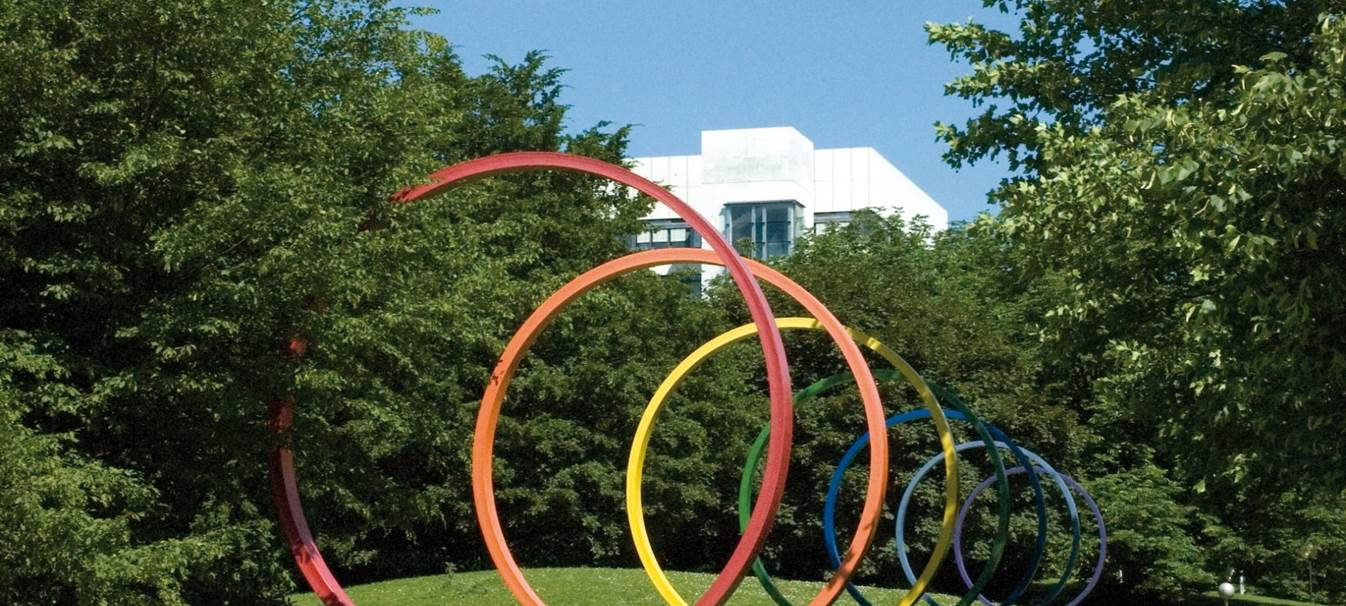
\includegraphics[width=0.7\textwidth]{images/tudo-title-2.jpg}}


\begin{document}
\maketitle
\begin{frame}
\end{frame}

\begin{frame}{Gliederung}
\begin{itemize}
  \item Stromnetz
  \begin{itemize}
  \item Vorderungen an das Stromnetz
  \item Frequenz im Netz
  \item Reguationsmechanismen der Frequenz
  \item Spannungsebenen
  \item Verteilung
  \item Netzbetreiber
  \item Anspruch an das Stromnetz durch die Energiewende
  \end{itemize}
\end{itemize}
\end{frame}
\begin{frame}
\begin{itemize}
 \item Strombörse
\begin{itemize}
  \item Enwicklung der Strombörse
  \item Angebote der Strombörse
  \item Spot Markt(und seine Folgen auf das Netz)
  \item Strompreis aus der Merit Order
  \item EEG-Umlage
  \item Strompreisentwicklung
\end{itemize}
\end{itemize}
\end{frame}


\begin{frame}{Stromnetz-Historisch}
\begin{itemize}
  \item Beginn der Elektrifizierung 1880 mit der Industrialisierung
  \item zunächst nur Inselnetze mit Gleichstrom zur Beleuchtung
  \item Wechselstrom setzte sich gegen Gleichstrom wegen Vorteilen wie
  \begin{itemize}
    \item[-] einfache Transformation der Spannung durch einen Transformator
    \item[$\rightarrow$] einfaches Umspannen auf Hochspannung möglich
    somit weniger Verluste bei langen Leitungen
    \item[-] große Verbundnetze möglich, die aber alle synchron mit gleicher Frequenz betrieben werden.
  \end{itemize}
  \item heute nur vereinzelt Gleichstrom z. B. bei Verkehr und HGÜ
\end{itemize}
\end{frame}

{
\setbeamertemplate{footline}{}
\begin{frame}{Europäisches Verbundsystem}
\begin{columns}
\begin{column}{0.5\textwidth}
\begin{itemize}
  \item besteht aus mehrere voneinander getrennte Verbundsysteme
\item Verbundsystem
Zusammenschluss von Höchst und Hochspannungsnetzen der Länder zur z. B. UCT  (Union for the Co-ordination of the Transmission of Electricity)
  \item Verband Europäischer Übertragungsnetzbetreiber
   European Network of Transmission System (ENTSO-E) übernimmt Koordination
der Verbundsysteme
\end{itemize}
\end{column}
\begin{column}{0.5\textwidth}
    \begin{figure}
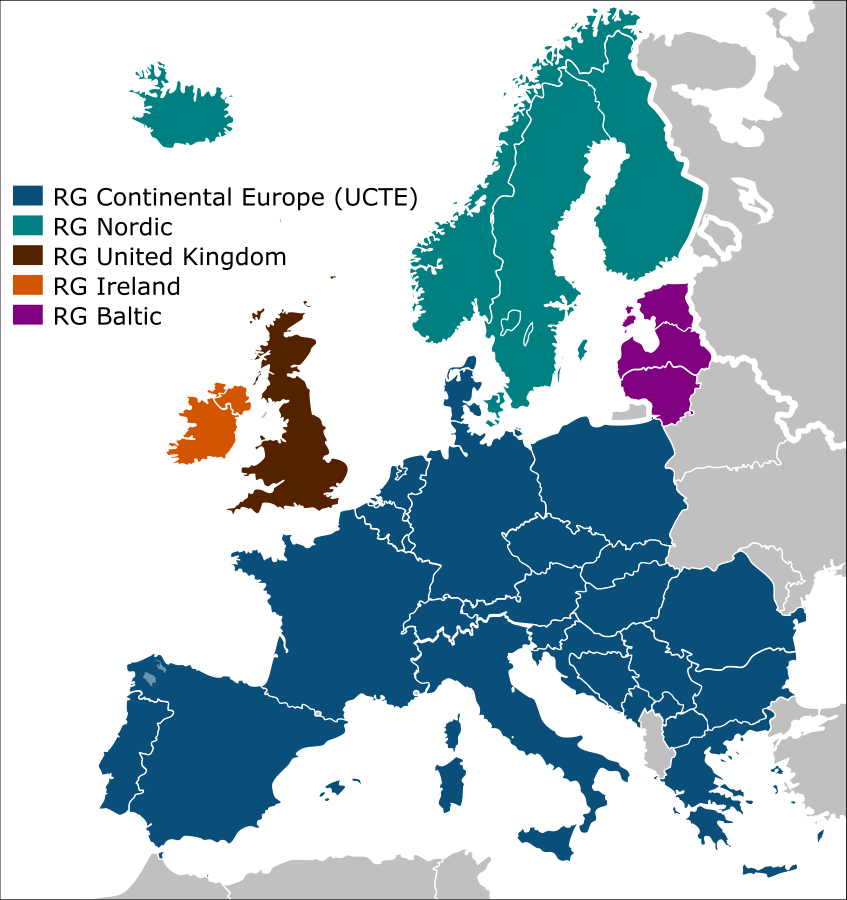
\includegraphics[width=0.9\textwidth]{images/Euronetz.png}
\end{figure}
\end{column}
\end{columns}
% Quelle: https://commons.wikimedia.org/w/index.php?curid=1387849
\end{frame}
}

\begin{frame}
  \begin{block}{Hochspannungs-Gleichstrom-Übertragung (HGÜ)}
    \begin{itemize}
      \item dient zur Energieübertragung zwischen zwei weit entfernten Punkten
      \item ab $\SI{750}{\kilo\meter}$ effizienter als Leitungen mit Wechselstrom
  \item[] \textbf{\textcolor{tugreen}{Ursache:}} HGÜ: ohmscher Widerstand
  \item[] \textbf{\textcolor{tulight}{Ursache:}} Wechselstrom: ohmscher Widerstand, Skin-Effekt und Blindwiderstand
% \begin{tabular}{c c}
%  AC    &          DC \\
% \hline
% \multicolumn{2}{c}{OhmscherWiderstand}\\
% Skin-Effekt &  - \\
% BlindWiderstand& -\\
%  \end{tabular}
% \begin{itemize}
      \item verbindet die getrennten und asynchronen Verbundsysteme Europas und bspw. Offshore-Windparks mit dem Festland
      \end{itemize}
\end{block}

 \end{frame}

{
\setbeamertemplate{footline}{}
\begin{frame}
  \begin{columns}
\begin{column}{0.5\textwidth}
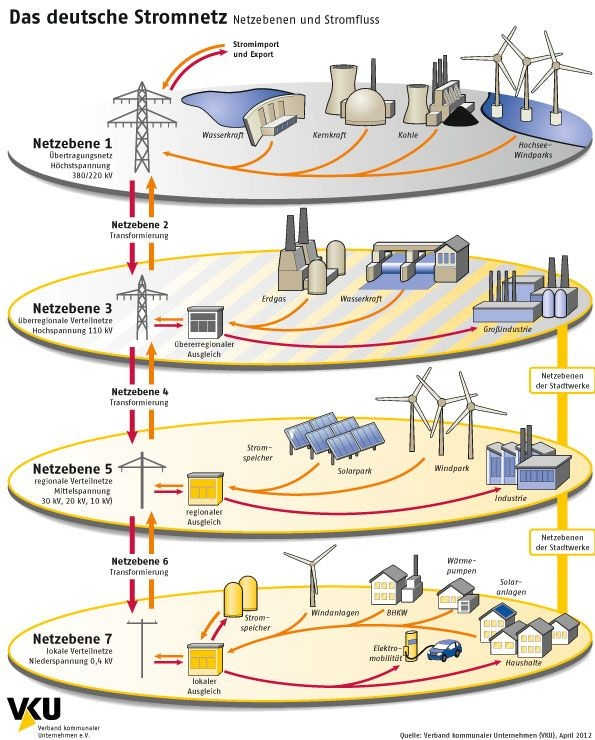
\includegraphics[width=1\textwidth]{images/netzebenen.jpg}
%Quelle: http://www.bpb.de/politik/wirtschaft/energiepolitik/148524/ausbau-des-stromnetzes
\end{column}
\begin{column}{0.5\textwidth}
  %\frametitle{Netzebenen}
  \begin{itemize}
    \item besteht aus \num{7} Netzebenen
    \item \num{4} Spannungsebenen
    \begin{itemize}
      \item[-] Höchstspannung $\num{220}$-$\SI{380}{\kilo\volt}$
      \item[-] Hochspannung  $\num{60}$-$\SI{110}{\kilo\volt}$
      \item[-] Mittelspannung  $\num{6}$-$\SI{50}{\kilo\volt}$
      \item[-] Niederspannung $\num{230}$/$\SI{400}{\volt}$
    \end{itemize}
    \item \num{3} Transformationsebenen jeweils zwischen den Spannungsebenen
  \end{itemize}
\end{column}
\end{columns}
\end{frame}
}


{
\setbeamertemplate{footline}{}
\begin{frame}
\begin{figure}
  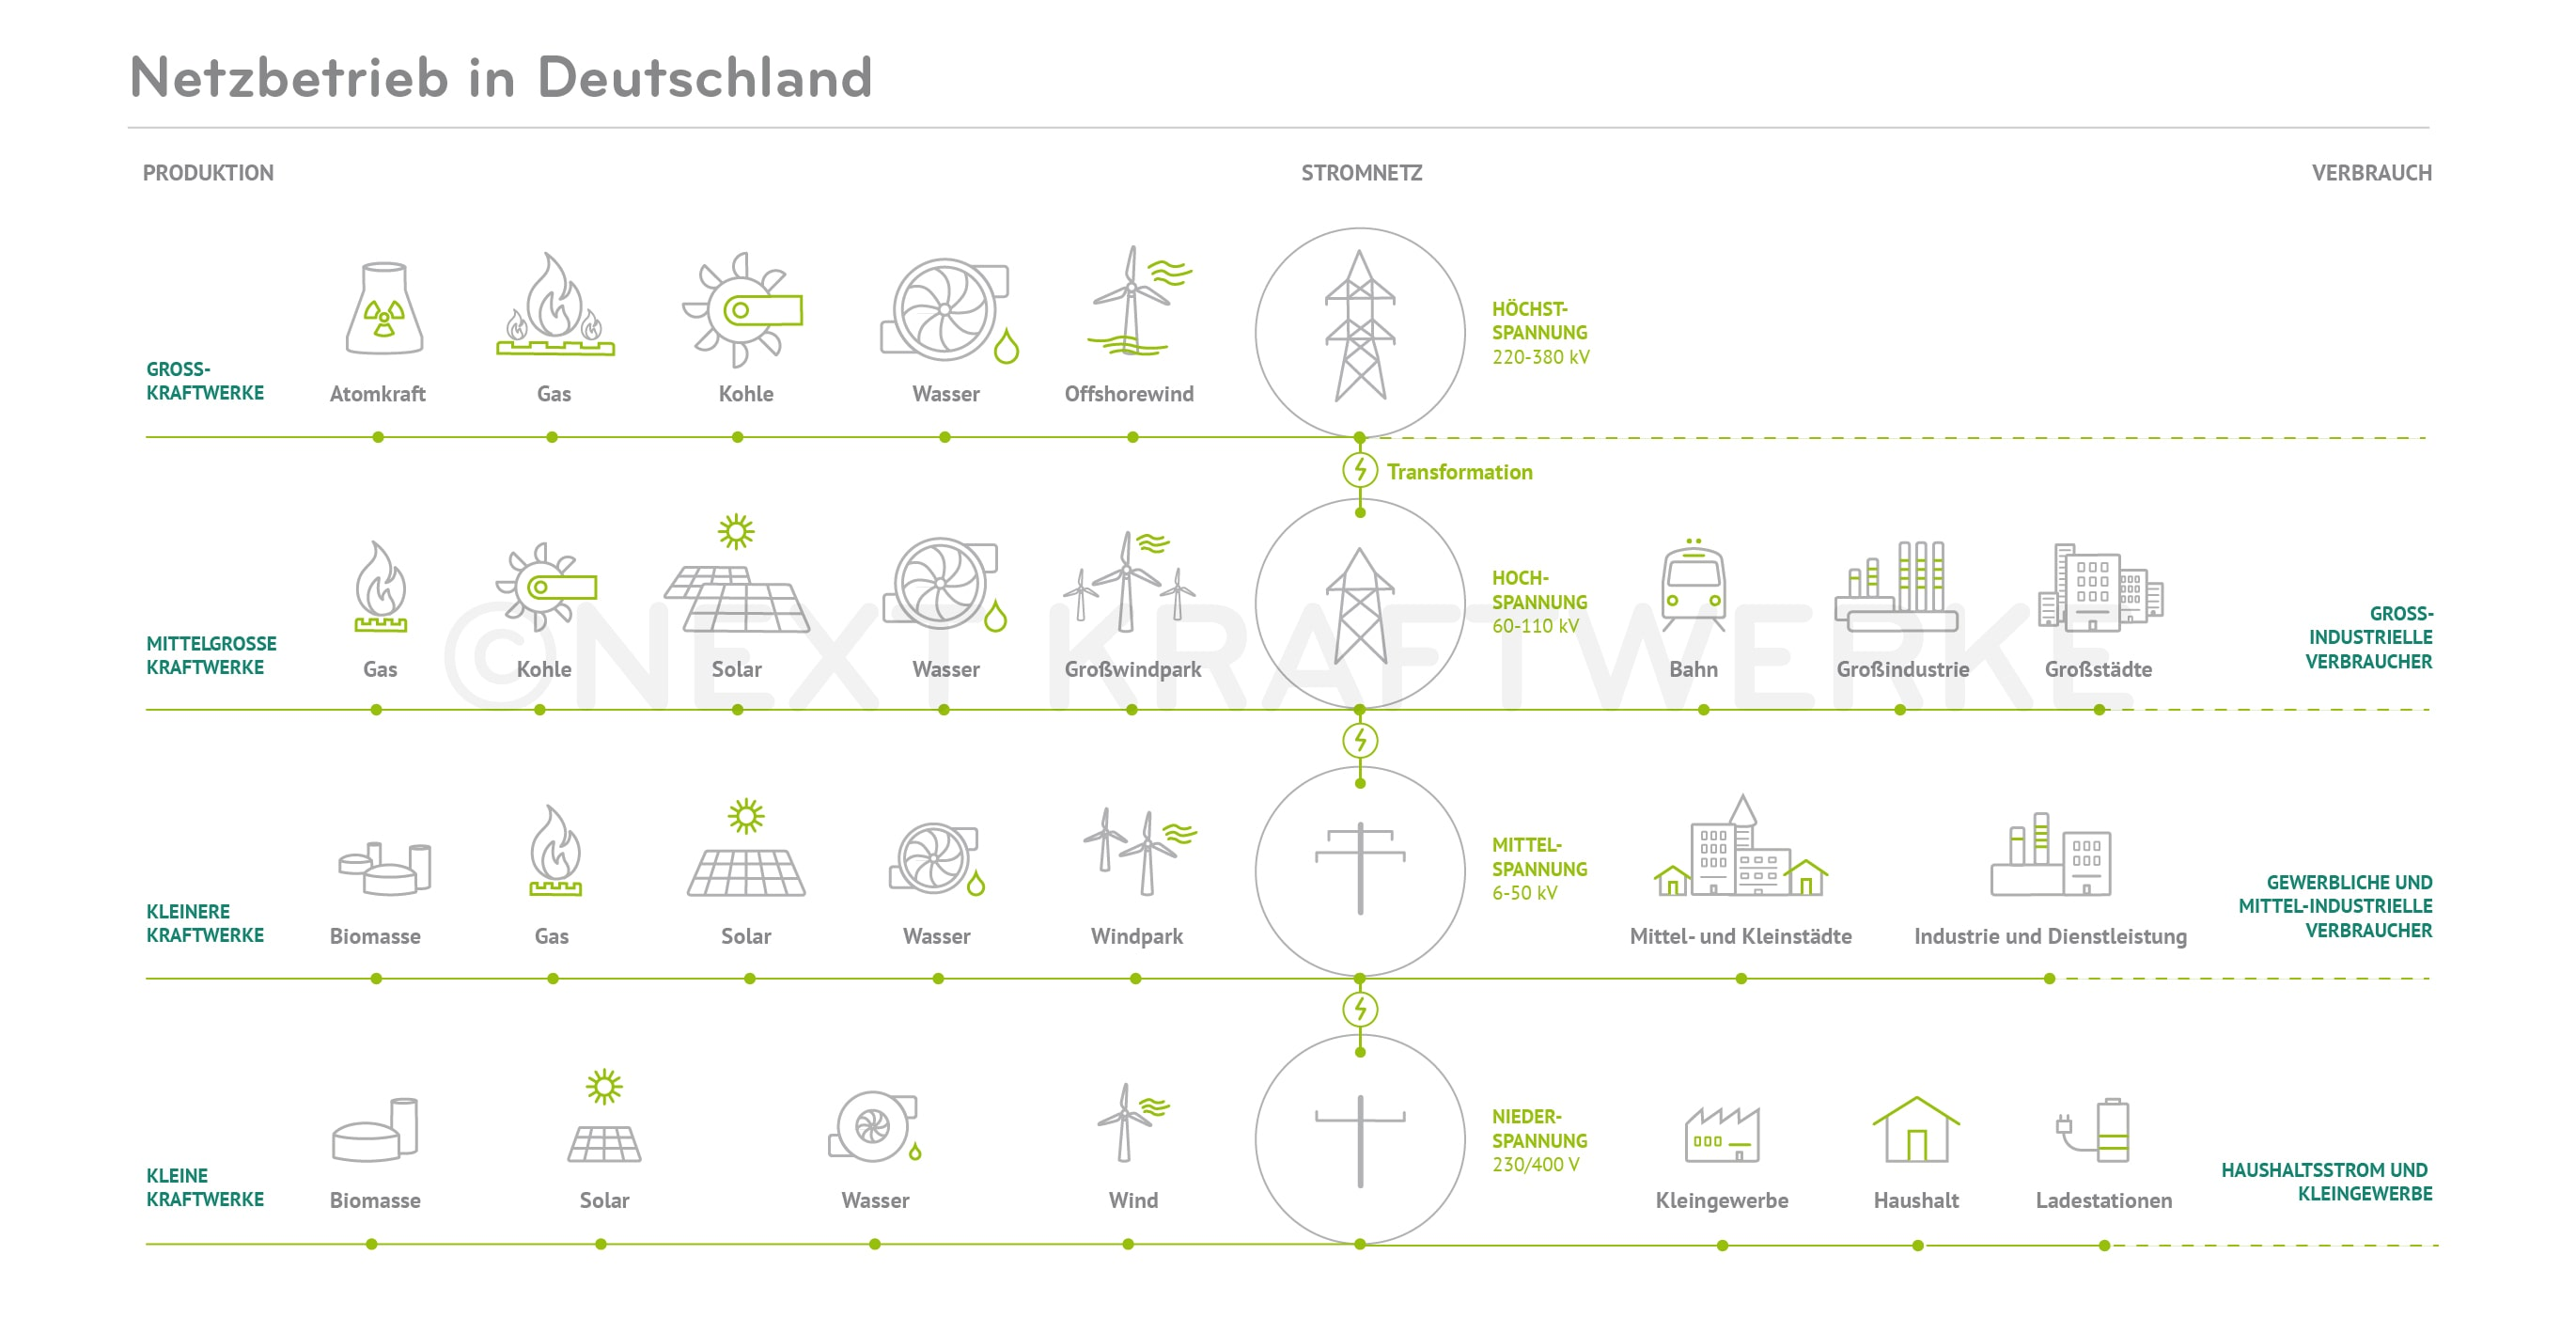
\includegraphics[width=1\textwidth]{images/netzbetrieb-deutsches-stromnetz.jpg}
\end{figure}
%:Quelle:
\end{frame}
}

\begin{frame}
  \begin{columns}
    \begin{column}{0.5\textwidth}
  \begin{itemize}
    \item Hoch-/Mittel-/Niederspannungs Ebenen
     werden regional und lokal von Verteilernetzbetreibern verwaltet
    \item die Höchstspannung Ebene teilen sich in
    Deutschland die Übertragungsnetzbetreiber
    \begin{itemize}
      \item[-] Tennet
      \item[-] 50-Hertz
      \item[-] Amprion
      \item[-] Transnet
  \end{itemize}
\end{itemize}
\end{column}
\begin{column}{0.5\textwidth}
\begin{figure}
    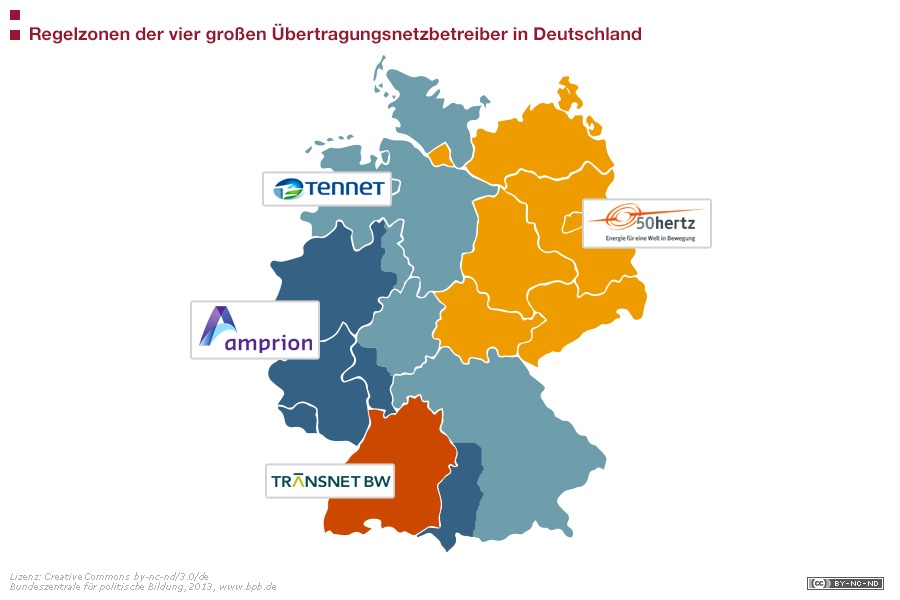
\includegraphics[width=1\textwidth]{images/UNB.jpg}
%Quelle:http://www.bpb.de/politik/wirtschaft/energiepolitik/148524/ausbau-des-stromnetzes
\end{figure}
\end{column}
\end{columns}
\end{frame}

\begin{frame}{Netzfrequenz}
\begin{itemize}% [<+->]
\item Richtfrequenz von $\SI{50}{\hertz}$ im europäischen Verbundnetz
\item hängt von Rotationsgeschwindigkeit der synchronisierten Generatoren
ab
% Um dieses umgangssprachlicher zu erklären, wird
% gerne der Alltagsvergleich mit einem Fahrrad herangezogen:
% Auf einer gleichmässigen Fläche kann relativ einfach eine
% konstante Trittgeschwindigkeit gehalten werden.
% An einer Steigung (zu vergleichen mit steigender Last im Stromnetz)
% muss mehr Kraft aufgewendet werden, um die Trittfrequenz
% beizubehalten oder sie kann sogar (kurzeitig) sinken,
% bis man sich auf die Steigung eingestellt hat.
% Anders herum steigt die (Tritt-)Frequenz an einem Gefälle
% kurz an, bis man sie (zum Beispiel durch Bremsen) wieder
% auf die „normale“ Nennfrequenz gesenkt hat.
\item Zu starke Abweichungen können Zerstörung der Generatoren und anderen Geräten führen
% \begin{itemize}[<+->]
%   \item test ...
%   \item test 2
% \end{itemize}
%führen
\item im Stromnetz kann keine Energie gespeichert werden
  \begin{itemize}
    \item[\rightarrow]  erzeugter Leistung $\stackrel{!}{=}$ abgenommene Leistung 
  \end{itemize}
  \item Schwankungen in
  der Relation von abgenommener und erzeugter Leistung erzeugt Abweichungen in der Frequenz
\end{itemize}
\end{frame}

{
\setbeamertemplate{footline}{}
\begin{frame}
  \begin{figure}
  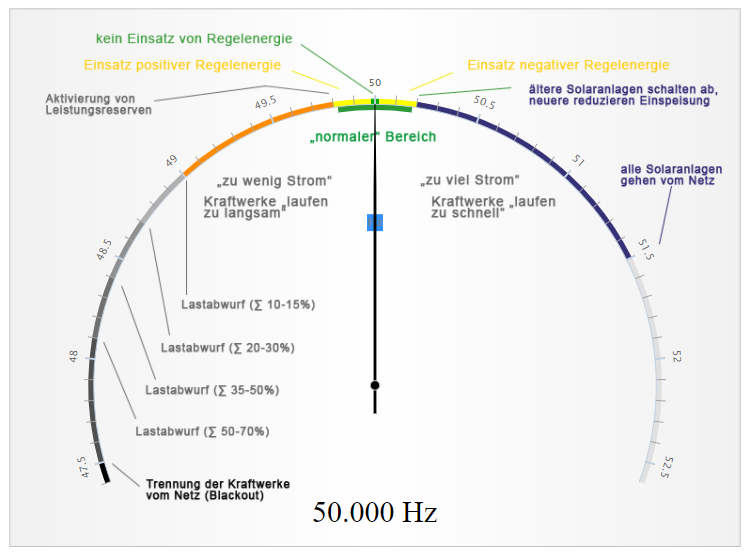
\includegraphics[width=0.9\textwidth]{images/Frequenz.png}
  \end{figure}
%Quelle:http://www.netzfrequenz.info/aktuelle-netzfrequenz-full
\end{frame}
}

\begin{frame}{Regelung der Netzfrequenz}
Notwendigkeit von Regelbarer Leistung um Frequenz konstant zu halten
\begin{itemize}
  \item positive Regelenergie:
  \begin{itemize}
    \item[-] mehr Strom muss in das Netz eingespeist werden
    \item[-] weniger Strom muss verbraucht werden
  \end{itemize}
  \item negative Regelenergie:
  \begin{itemize}
    \item[-] Stromeinspeisung muss schnell reduziert werden
    \item[-] mehr Strom muss verbraucht werden
  \end{itemize}
  \item[\rightarrow] Kraftwerke oder Verbraucher mit einer diesen Eigenschaften eignen sich um Regelenergie bereitzustellen
\end{itemize}
\end{frame}

\begin{frame}
  \begin{itemize}
    \item Primärregelung PRL
    \begin{itemize}
      \item[-] automatische vollständige Aktivierung innerhalb von \SI{30}{\second}
      \item[-] abzudeckender Zeitraum \num{0}<\SI{15}{\minute}
      \item[-] Bereitstellung durch alle ÜNB im ENTSO-E-Gebiet
      \item[-] Frequenzabhängige Lasten Vorteilhaft z. B. ?Asynchronmotor?
      \item[-] ?keine Unterscheidung zwischen positiver und negativer Regelenergie?
    \end{itemize}
    \item Sekundärregelung SRL
    \begin{itemize}
      \item[-] automatische Aktivierung durch betroffenen ÜNB
      \item[-] vollständige Aktivierung innerhalb von \SI{5}{\minute}
      \item[-] Unterscheidung zwischen positiver und negativer Regelenergie
      \item[-] Breitstellung durch z. B. Pumpspeicherkraftwerken, Gasturbinen, Biogasanlagen oder Blockheizkraftwerke
    \end{itemize}
    \item Tertiärregelung(Minutenreserve) MRL
    \begin{itemize}
      \item[-] Aktivierung innerhalb von \SI{15}{\minute}
      \item[-] abzudeckender Zeitraum mehrere Stunden bei Störungen
      \item[-] Unterscheidung zwischen positiver und negativer Regelenergie
      \item[-] Breitstellung durch Kraftwerke identisch zu SRL oder Verbraucher deren Lasten abgeworfen werden
    \end{itemize}
  \end{itemize}

\end{frame}


{
\setbeamertemplate{footline}{}
\begin{frame}
  \begin{figure}
  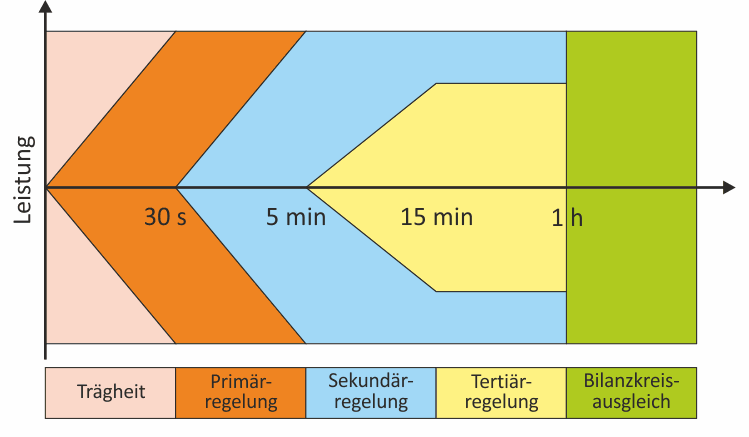
\includegraphics[width=0.9\textwidth]{images/Regelleistung.png}
\end{figure}
%Quelle:https://fenecon.de/page/stromspeicher-energy-pool
\end{frame}
}

\begin{frame}{Energiewende und folgen im Stromnetz}
  \begin{columns}
  \begin{column}{0.5\textwidth}
konventionelles Stromnetz:
\begin{itemize}
  \item Kraftwerkleistungen werden an Lastprofil angepasst
  \item "Einbahnstraße im Stromnetz" Kraftwerk$\rightarrow$Verbraucher
Höchspannung$\rightarrow$Niederspannung
\end{itemize}
  \end{column}
  \begin{column}{0.5\textwidth}
neues Stromnetz:
\begin{itemize}
\item EE-Kraftwerkleistungen nur noch bedingt (z.B Wasser) oder gar nicht (z.B Wind/Sonne) steuerbar
\begin{itemize}
  \item[$\rightarrow$] keine Anpassung an Lastprofil möglich
\end{itemize}
\item durch erneuerbare Energiequellen  Höchstspannung$\leftrightarrows$Niederspannung
\end{itemize}
\end{column}
\end{columns}
\textbf{\textcolor{tugreen}{Fazit:}} Notwendigkeit des Netz-um/aus-bau durch Energiewende
\end{frame}

\begin{frame}{Netzausbau}

\end{frame}
\begin{frame}{Blackout}
!!!!!!!!!!!!!!!!!!!!!!!!!!!!!!!!!!
\end{frame}




\begin{frame}{Strombörse}
\begin{itemize}
  \item existiert seit \num{2000} in Europa
  \item Strombörsen in Europa koordiniert von der EEX Group
  \item Deutschland, Frankreich, Österreich
  und Schweiz handeln an European Energy Exchange (EEX) in Leipzig
 und European Power Exchange (EPEX SPOT) in Paris
 \item Unterscheidung zwischen Spotmarkt, Terminmarkt und Regelenergiemarkt
\item Gehandelte Produkte zusätzlich zu Strom:
    \begin{itemize}
      \item[-]Öl, Gas, Kohle, Metall, Frachtprodukte,
       Emissionsberechtigungen sowie Agrarprodukte
    \end{itemize}
\end{itemize}
\end{frame}


{
\setbeamertemplate{footline}{}
\begin{frame}
  \begin{figure}
  \includegraphics[width=1.1\textwidth]{images/stromprodukte.jpg}
\end{figure}
%Quelle:https://www.next-kraftwerke.de/wissen/strommarkt/spotmarkt-epex-spot
\end{frame}
}

\begin{frame}{Spotmarkt}
  \begin{itemize}
    \item Spotmarkt in Paris an der EPEX SPOT
    \item Handel von kurzfristig lieferbaren Strommengen in bestimmten Blöcken
    \item Im Intraday-Handel (Lieferung am selben Tag)
    \item Im Day-Ahead-Handel (Lieferung am Folgetag)
  \end{itemize}
\end{frame}

\begin{frame}{Merit-Order}
\begin{itemize}
  \item Beschreibungsmodell der Preisbildung auf dem Strommarkt
  \item orientiert sich an den Grenzkosten der Kraftwerke
  (Grenzkosten entspricht kosten für die letzte produzierte Megawattstunde)
\item Kraftwerke mit niedrigen Grenzkosten werden bei der
 Einspeisung bevorzugt, bis Nachfrage gedeckt ist
\item Börsenpreis ergibt sich aus Schnittstelle von Angebot und Nachfrage
\begin{itemize}
  \item[$\rightarrow$] Grenzkosten des Kraftwerkes, welches zuletzt den
  Zuschlag zur Einspeisung erhält, definiert Börsenpreis für alle eingespeisten Kraftwerke("uniform pricing")
\end{itemize}
\end{itemize}
\end{frame}

{
\setbeamertemplate{footline}{}
\begin{frame}
  \begin{figure}
  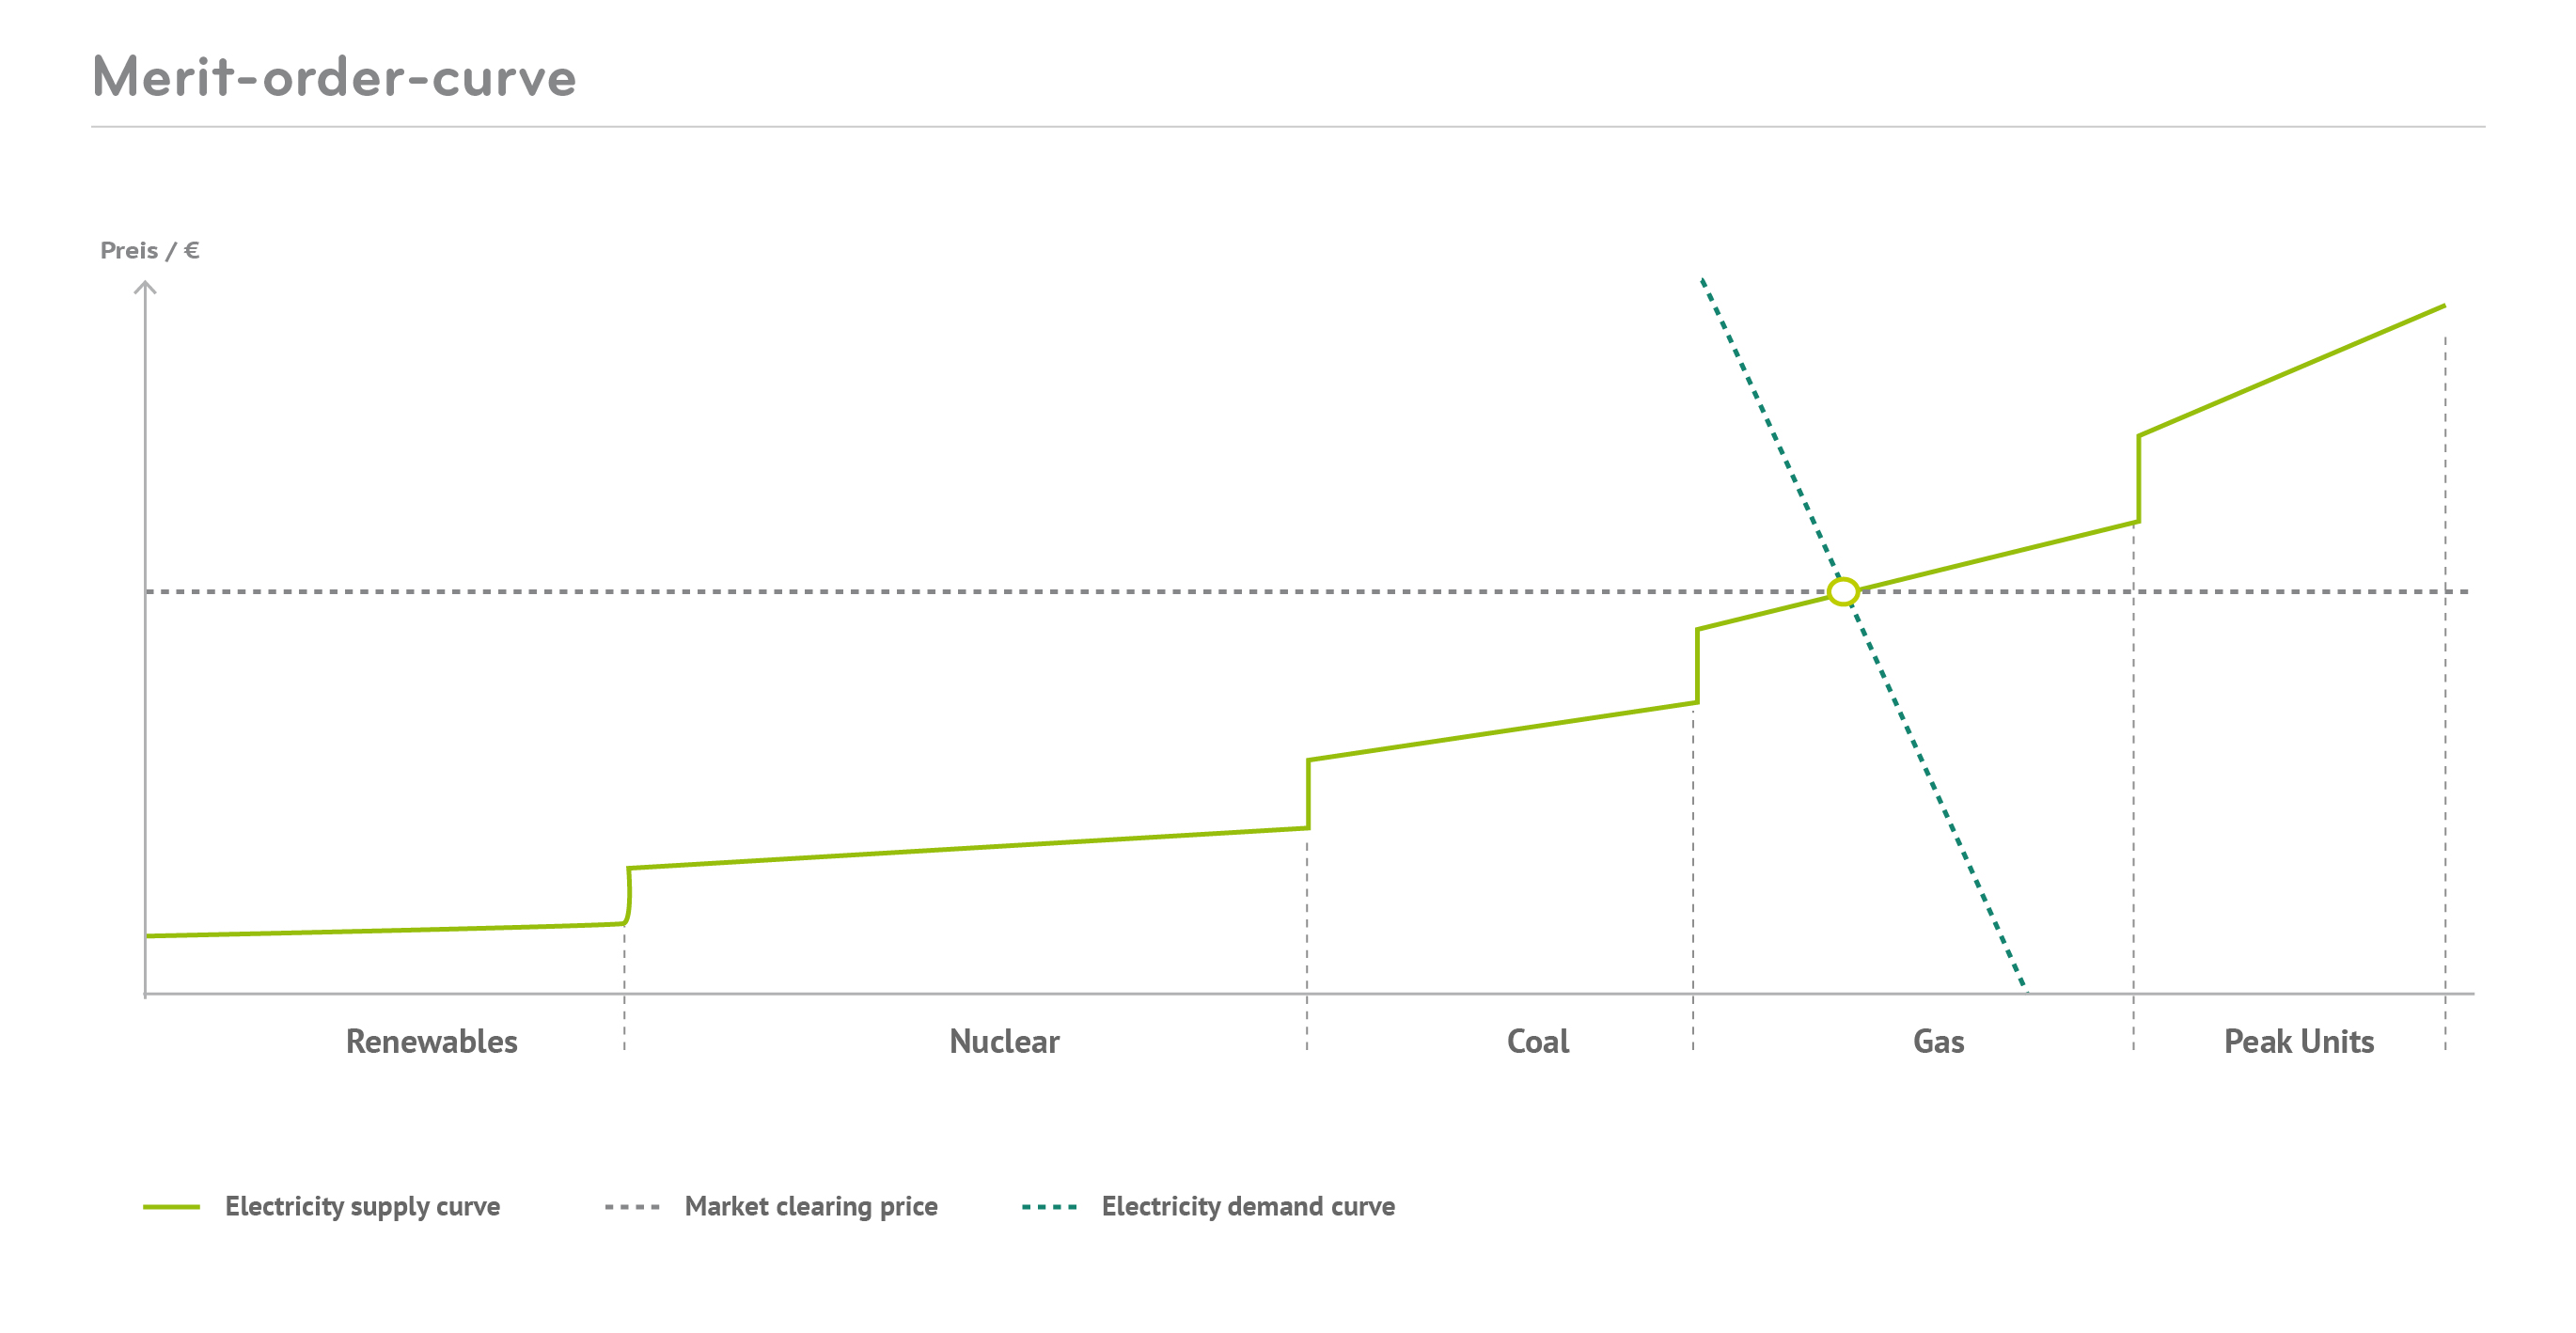
\includegraphics[width=1\textwidth]{images/Merit-order-curve-2.jpg}
\end{figure}
%Quelle:https://www.next-kraftwerke.be
\end{frame}
}

{
\setbeamertemplate{footline}{}
\begin{frame}
  \begin{figure}
  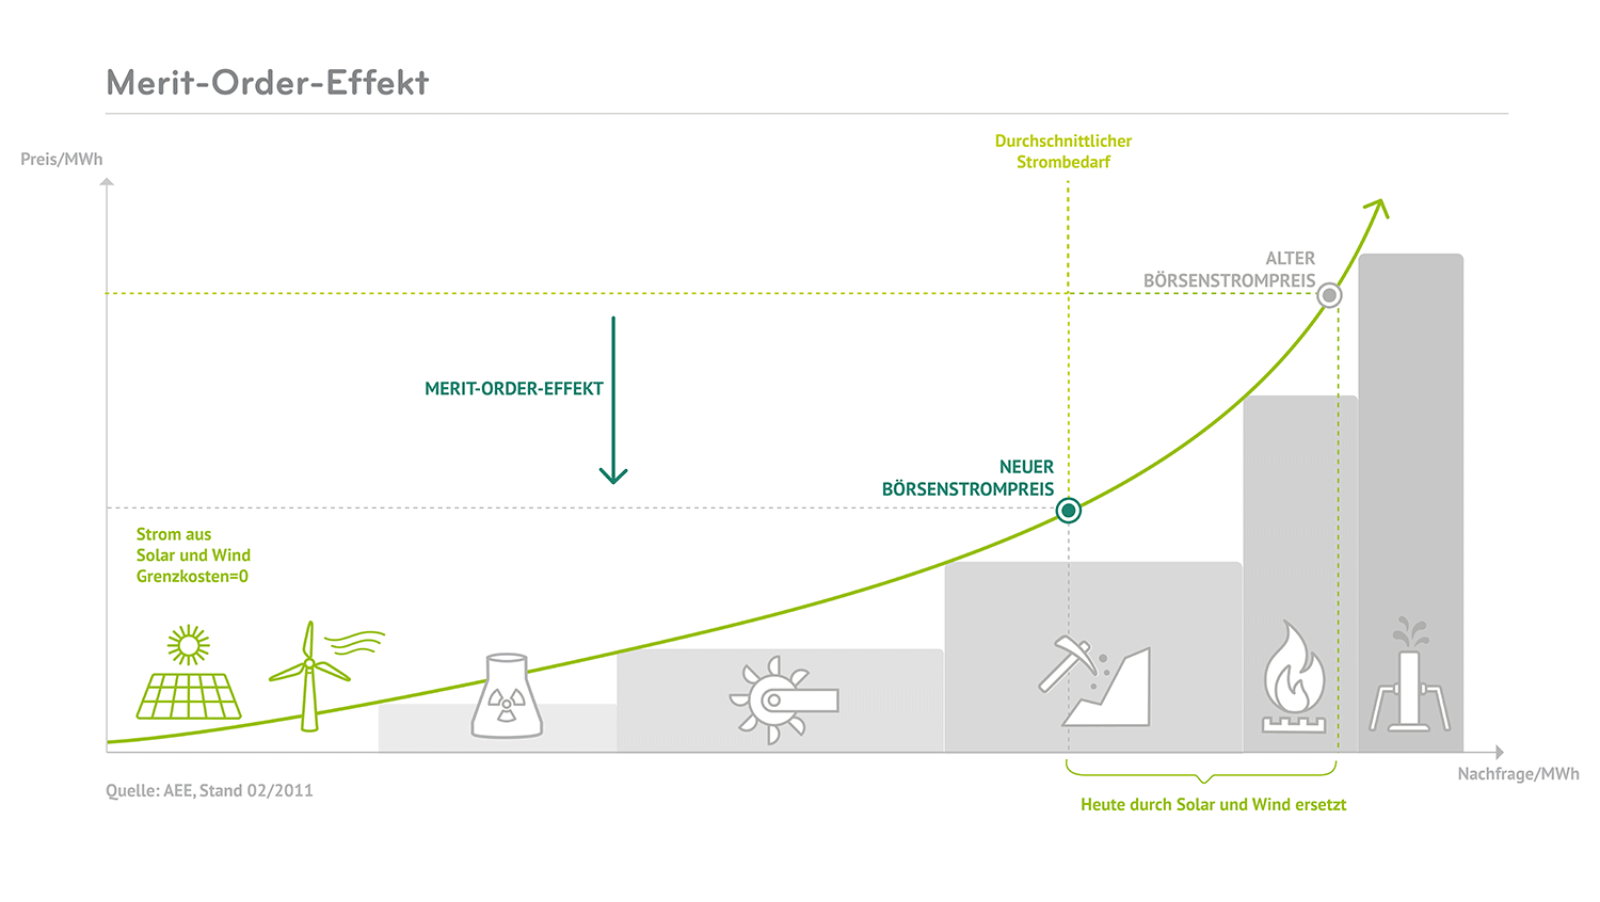
\includegraphics[width=1\textwidth]{images/Merit.png}
\end{figure}
%Quelle:https://www.next-kraftwerke.be
\end{frame}
}

\begin{frame}{Terminmarkt}
\begin{itemize}
  \item Terminmarkt in Leipzig an der EEX
  \item Handel von Strommengen, die zu einem festen Termin zu Verfügung gestellt werden (Strom-Futures)
  \item bis zu 6 Jahre Strom im voraus kaufen
  \item Jahr-, Quartal-, Monat-, Woche-,  Wochenende- und Tag-Kontrakte
  \item Preis richtig sich an Börsenindex der Strombörse z. B. Phelix (Physical Electricity Index)
\end{itemize}
\end{frame}

\begin{frame}{Regelenergiemarkt}
\begin{itemize}
  \item Bedarf an Regelenergien von PRL, SRL und MRL werden durch Ausschreibung
der ÜNB gedeckt
\item PRL und SRL werden jede Woche neu ausgeschrieben
\item MRL werden Täglich neu ausgeschrieben und nach Merit-Order-Liste bei Bedarf abgerufen
\item Preis für Regleenergien ??
\end{itemize}

\end{frame}
\begin{frame}{Erneuerbare-Energien-Gesetz EEG}
   \begin{itemize}
     \item das EEG wurde im Jahr 2000 eingeführt und mehrmals überarbeitet aktuell EEG 2017
   \end{itemize}
\pause
    \begin{block}{Ziel:}
      Förderung von Erneuerbaren Energiequellen, damit Umstieg von Konventionellen zur Erneuerbaren Energiequellen gelingt
    \end{block}
  %\item Regelt die Einspeisung des EE-Stromes
\pause
    \begin{block}{Maßnahmen des EEG zu Förderung von EE-Strom:}
     \begin{itemize}
       \item[$\rightarrow$] Verpflichtung an die Netzbetreiber EE-Anlagen an das Stromnetz anzuschießen und EE-Strom vorrangig einzuspeisen
       \item[$\rightarrow$] garantierte Einspeisevergütung des EE-Stromes an die Anlagenbetreiber durch den Netzbetreiber für 20 Jahre
   \end{itemize}
   \end{block}
\end{frame}

\begin{frame}{Auswirkungen des EEG}
  \begin{itemize}
    \item Abnahmepflicht fördert Merit-Order-Effekt
    \item Netzbetreiber bieten abgenommenen EE-Strom an der Börse an
\begin{itemize}
  \item[$\rightarrow$] Gewinn an der Strombörse deckt jedoch nicht die vollen Vergütungskosten der Netzbetreiber
\end{itemize}
\end{itemize}
\begin{block}{EEG-Umlage}
\begin{itemize}
  \item $\text{EEG-Umlage}=\text{Einspeisevergütung}-\text{Börsengewinn}$
\item die EEG-Umlage erhält der Netzbetreiber von allen Stromverbrauchern
\item Strompreis enthält die EEG-Umlage
\end{itemize}
\end{block}
\end{frame}

{
\setbeamertemplate{footline}{}
\begin{frame}
  \begin{figure}
  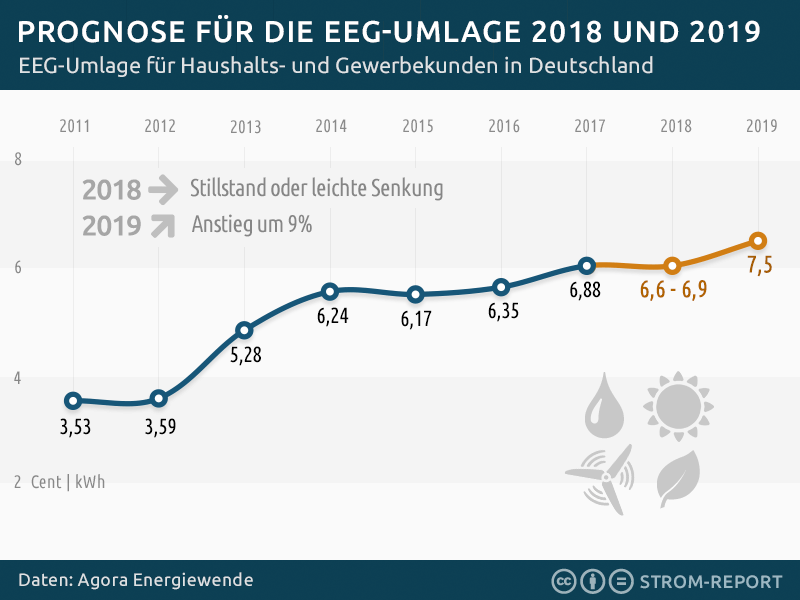
\includegraphics[width=0.9\textwidth]{images/eeg-umlage-2018-2019.png}
  \end{figure}
%Quelle:https://1-stromvergleich.com/strom-report/eeg-umlage/#eeg-umlage-2018
\end{frame}
}




{
\setbeamertemplate{footline}{}
\begin{frame}
  \begin{figure}
  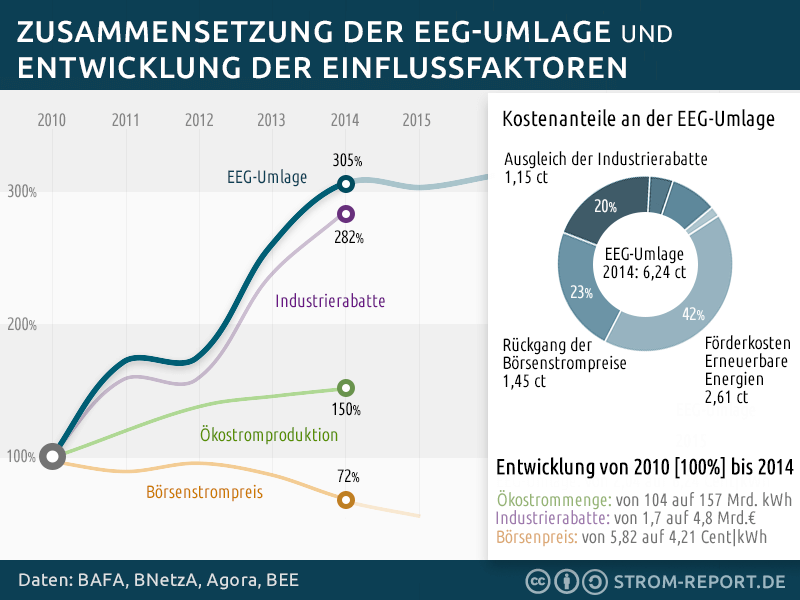
\includegraphics[width=0.9\textwidth]{images/eeg-umlage.png}
  \end{figure}
%Quelle:https://1-stromvergleich.com/strom-report/eeg-umlage/#eeg-umlage-boersenpreis-industrierabatt
\end{frame}
}


\begin{frame}{Entwicklung}

\end{frame}
\end{document}


\begin{frame}{Paradigmenwechsel}

\end{frame}


\begin{frame}{Backup}

\end{frame}

{
\setbeamertemplate{footline}{}
\begin{frame}
  \begin{figure}
  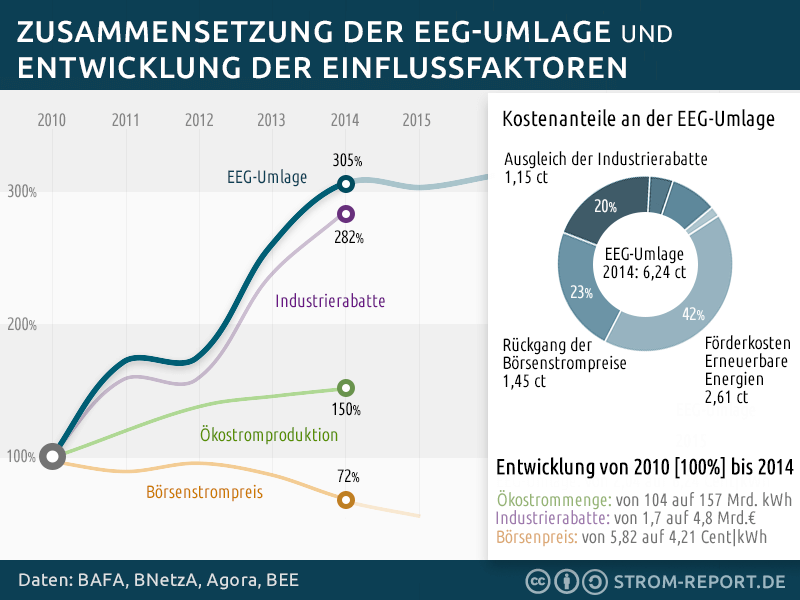
\includegraphics[width=0.9\textwidth]{images/eeg-umlage.png}
  \end{figure}
%Quelle:https://1-stromvergleich.com/strom-report/eeg-umlage/#eeg-umlage-boersenpreis-industrierabatt
\end{frame}
}
